\documentclass[twoside]{book}

% Packages required by doxygen
\usepackage{fixltx2e}
\usepackage{calc}
\usepackage{doxygen}
\usepackage[export]{adjustbox} % also loads graphicx
\usepackage{graphicx}
\usepackage[utf8]{inputenc}
\usepackage{makeidx}
\usepackage{multicol}
\usepackage{multirow}
\PassOptionsToPackage{warn}{textcomp}
\usepackage{textcomp}
\usepackage[nointegrals]{wasysym}
\usepackage[table]{xcolor}

% Font selection
\usepackage[T1]{fontenc}
\usepackage[scaled=.90]{helvet}
\usepackage{courier}
\usepackage{amssymb}
\usepackage{sectsty}
\renewcommand{\familydefault}{\sfdefault}
\allsectionsfont{%
  \fontseries{bc}\selectfont%
  \color{darkgray}%
}
\renewcommand{\DoxyLabelFont}{%
  \fontseries{bc}\selectfont%
  \color{darkgray}%
}
\newcommand{\+}{\discretionary{\mbox{\scriptsize$\hookleftarrow$}}{}{}}

% Page & text layout
\usepackage{geometry}
\geometry{%
  a4paper,%
  top=2.5cm,%
  bottom=2.5cm,%
  left=2.5cm,%
  right=2.5cm%
}
\tolerance=750
\hfuzz=15pt
\hbadness=750
\setlength{\emergencystretch}{15pt}
\setlength{\parindent}{0cm}
\setlength{\parskip}{3ex plus 2ex minus 2ex}
\makeatletter
\renewcommand{\paragraph}{%
  \@startsection{paragraph}{4}{0ex}{-1.0ex}{1.0ex}{%
    \normalfont\normalsize\bfseries\SS@parafont%
  }%
}
\renewcommand{\subparagraph}{%
  \@startsection{subparagraph}{5}{0ex}{-1.0ex}{1.0ex}{%
    \normalfont\normalsize\bfseries\SS@subparafont%
  }%
}
\makeatother

% Headers & footers
\usepackage{fancyhdr}
\pagestyle{fancyplain}
\fancyhead[LE]{\fancyplain{}{\bfseries\thepage}}
\fancyhead[CE]{\fancyplain{}{}}
\fancyhead[RE]{\fancyplain{}{\bfseries\leftmark}}
\fancyhead[LO]{\fancyplain{}{\bfseries\rightmark}}
\fancyhead[CO]{\fancyplain{}{}}
\fancyhead[RO]{\fancyplain{}{\bfseries\thepage}}
\fancyfoot[LE]{\fancyplain{}{}}
\fancyfoot[CE]{\fancyplain{}{}}
\fancyfoot[RE]{\fancyplain{}{\bfseries\scriptsize Generated by Doxygen }}
\fancyfoot[LO]{\fancyplain{}{\bfseries\scriptsize Generated by Doxygen }}
\fancyfoot[CO]{\fancyplain{}{}}
\fancyfoot[RO]{\fancyplain{}{}}
\renewcommand{\footrulewidth}{0.4pt}
\renewcommand{\chaptermark}[1]{%
  \markboth{#1}{}%
}
\renewcommand{\sectionmark}[1]{%
  \markright{\thesection\ #1}%
}

% Indices & bibliography
\usepackage{natbib}
\usepackage[titles]{tocloft}
\setcounter{tocdepth}{3}
\setcounter{secnumdepth}{5}
\makeindex

% Hyperlinks (required, but should be loaded last)
\usepackage{ifpdf}
\ifpdf
  \usepackage[pdftex,pagebackref=true]{hyperref}
\else
  \usepackage[ps2pdf,pagebackref=true]{hyperref}
\fi
\hypersetup{%
  colorlinks=true,%
  linkcolor=blue,%
  citecolor=blue,%
  unicode%
}

% Custom commands
\newcommand{\clearemptydoublepage}{%
  \newpage{\pagestyle{empty}\cleardoublepage}%
}

\usepackage{caption}
\captionsetup{labelsep=space,justification=centering,font={bf},singlelinecheck=off,skip=4pt,position=top}

%===== C O N T E N T S =====

\begin{document}

% Titlepage & ToC
\hypersetup{pageanchor=false,
             bookmarksnumbered=true,
             pdfencoding=unicode
            }
\pagenumbering{alph}
\begin{titlepage}
\vspace*{7cm}
\begin{center}%
{\Large Evaluator }\\
\vspace*{1cm}
{\large Generated by Doxygen 1.8.13}\\
\end{center}
\end{titlepage}
\clearemptydoublepage
\pagenumbering{roman}
\tableofcontents
\clearemptydoublepage
\pagenumbering{arabic}
\hypersetup{pageanchor=true}

%--- Begin generated contents ---
\chapter{Class Index}
\section{Class List}
Here are the classes, structs, unions and interfaces with brief descriptions\+:\begin{DoxyCompactList}
\item\contentsline{section}{\hyperlink{classBinTree}{Bin\+Tree$<$ T $>$} }{\pageref{classBinTree}}{}
\item\contentsline{section}{\hyperlink{classCourse}{Course} \\*Repository of \hyperlink{classSession}{Session} instances identified by an unique id }{\pageref{classCourse}}{}
\item\contentsline{section}{\hyperlink{classCourses}{Courses} \\*Interface of a repository of different courses, uniquely identified by their id }{\pageref{classCourses}}{}
\item\contentsline{section}{\hyperlink{classEvaluator}{Evaluator} \\*Class that contains a deployable instance of the \hyperlink{classEvaluator}{Evaluator} Platform }{\pageref{classEvaluator}}{}
\item\contentsline{section}{\hyperlink{classProblem}{Problem} \\*Class that behaves as an uniquely id-\/identified problem in the \hyperlink{classEvaluator}{Evaluator} platform }{\pageref{classProblem}}{}
\item\contentsline{section}{\hyperlink{classProblem__repo}{Problem\+\_\+repo} \\*General interface for a repository of \hyperlink{classProblem}{Problem} instances }{\pageref{classProblem__repo}}{}
\item\contentsline{section}{\hyperlink{classSession}{Session} \\*Class that behaves as a problem set with completion requisites }{\pageref{classSession}}{}
\item\contentsline{section}{\hyperlink{classSessions}{Sessions} \\*General interface to manage a \hyperlink{classSession}{Session} repository }{\pageref{classSessions}}{}
\item\contentsline{section}{\hyperlink{classUsers}{Users} \\*General interface to store and access the user list }{\pageref{classUsers}}{}
\end{DoxyCompactList}

\chapter{File Index}
\section{File List}
Here is a list of all documented files with brief descriptions\+:\begin{DoxyCompactList}
\item\contentsline{section}{src/include/{\bfseries Bin\+Tree.\+hh} }{\pageref{BinTree_8hh}}{}
\item\contentsline{section}{src/include/\hyperlink{commands_8hh}{commands.\+hh} \\*\hyperlink{classEvaluator}{Evaluator} main program class }{\pageref{commands_8hh}}{}
\item\contentsline{section}{src/include/\hyperlink{courses_8hh}{courses.\+hh} \\*\hyperlink{classCourse}{Course} class and its list interface }{\pageref{courses_8hh}}{}
\item\contentsline{section}{src/include/\hyperlink{problems_8hh}{problems.\+hh} \\*\hyperlink{classProblem}{Problem} class and a problem repository interface }{\pageref{problems_8hh}}{}
\item\contentsline{section}{src/include/\hyperlink{sessions_8hh}{sessions.\+hh} \\*\hyperlink{classSession}{Session} class and the session list interface }{\pageref{sessions_8hh}}{}
\item\contentsline{section}{src/include/\hyperlink{users_8hh}{users.\+hh} \\*Specification of the whole User list/\+DB general-\/use interface }{\pageref{users_8hh}}{}
\end{DoxyCompactList}

\chapter{Class Documentation}
\hypertarget{classBinTree}{}\section{Bin\+Tree$<$ T $>$ Class Template Reference}
\label{classBinTree}\index{Bin\+Tree$<$ T $>$@{Bin\+Tree$<$ T $>$}}
\subsection*{Public Member Functions}
\begin{DoxyCompactItemize}
\item 
\mbox{\Hypertarget{classBinTree_a1ab686e0bcf990093ff91fe71744c1a4}\label{classBinTree_a1ab686e0bcf990093ff91fe71744c1a4}} 
{\bfseries Bin\+Tree} (const T \&x)
\item 
\mbox{\Hypertarget{classBinTree_adb7eeff76d08130c943b36af215eb521}\label{classBinTree_adb7eeff76d08130c943b36af215eb521}} 
{\bfseries Bin\+Tree} (const T \&x, const \hyperlink{classBinTree}{Bin\+Tree} \&left, const \hyperlink{classBinTree}{Bin\+Tree} \&right)
\item 
\mbox{\Hypertarget{classBinTree_a74cda259ba5c25b8ee38ed4dc33e4fad}\label{classBinTree_a74cda259ba5c25b8ee38ed4dc33e4fad}} 
bool {\bfseries empty} () const
\item 
\mbox{\Hypertarget{classBinTree_a82108db4c1b08d1f111027788c196d4e}\label{classBinTree_a82108db4c1b08d1f111027788c196d4e}} 
\hyperlink{classBinTree}{Bin\+Tree} {\bfseries left} () const
\item 
\mbox{\Hypertarget{classBinTree_aff8e96651b27284c329667b5ad3e4d0b}\label{classBinTree_aff8e96651b27284c329667b5ad3e4d0b}} 
\hyperlink{classBinTree}{Bin\+Tree} {\bfseries right} () const
\item 
\mbox{\Hypertarget{classBinTree_a734e785b089c87b49187ee7c58edf5f3}\label{classBinTree_a734e785b089c87b49187ee7c58edf5f3}} 
const T \& {\bfseries value} () const
\end{DoxyCompactItemize}


The documentation for this class was generated from the following file\+:\begin{DoxyCompactItemize}
\item 
src/include/Bin\+Tree.\+hh\end{DoxyCompactItemize}

\hypertarget{classCourse}{}\section{Course Class Reference}
\label{classCourse}\index{Course@{Course}}


Repository of \hyperlink{classSession}{Session} instances identified by an unique id.  




{\ttfamily \#include $<$courses.\+hh$>$}

\subsection*{Public Member Functions}
\begin{DoxyCompactItemize}
\item 
bool \hyperlink{classCourse_a3e2bd434ae266de10601112d808f5e15}{is\+\_\+legal} ()
\item 
string \hyperlink{classCourse_a37e52d8c02455bccec118d3ca95b8496}{find\+\_\+session\+\_\+id} (string target\+\_\+problem)
\item 
\mbox{\Hypertarget{classCourse_a92302590d57b2871c76b369b53404cfc}\label{classCourse_a92302590d57b2871c76b369b53404cfc}} 
\hyperlink{classSession}{Session} \& {\bfseries operator\mbox{[}$\,$\mbox{]}} (string)
\end{DoxyCompactItemize}


\subsection{Detailed Description}
Repository of \hyperlink{classSession}{Session} instances identified by an unique id. 

The \hyperlink{classCourse}{Course} class behaves as a wrapper of uniquely identified by an id combinations \hyperlink{classSession}{Session} instances. 

\subsection{Member Function Documentation}
\mbox{\Hypertarget{classCourse_a37e52d8c02455bccec118d3ca95b8496}\label{classCourse_a37e52d8c02455bccec118d3ca95b8496}} 
\index{Course@{Course}!find\+\_\+session\+\_\+id@{find\+\_\+session\+\_\+id}}
\index{find\+\_\+session\+\_\+id@{find\+\_\+session\+\_\+id}!Course@{Course}}
\subsubsection{\texorpdfstring{find\+\_\+session\+\_\+id()}{find\_session\_id()}}
{\footnotesize\ttfamily string Course\+::find\+\_\+session\+\_\+id (\begin{DoxyParamCaption}\item[{string}]{target\+\_\+problem }\end{DoxyParamCaption})}


\begin{DoxyParams}{Parameters}
{\em target\+\_\+problem} & The problem id to be searched. \\
\hline
\end{DoxyParams}
\begin{DoxyReturn}{Returns}
An std\+::string containing the id of the internal session that contains the given problem id. 
\end{DoxyReturn}
\mbox{\Hypertarget{classCourse_a3e2bd434ae266de10601112d808f5e15}\label{classCourse_a3e2bd434ae266de10601112d808f5e15}} 
\index{Course@{Course}!is\+\_\+legal@{is\+\_\+legal}}
\index{is\+\_\+legal@{is\+\_\+legal}!Course@{Course}}
\subsubsection{\texorpdfstring{is\+\_\+legal()}{is\_legal()}}
{\footnotesize\ttfamily bool Course\+::is\+\_\+legal (\begin{DoxyParamCaption}{ }\end{DoxyParamCaption})}

\begin{DoxyReturn}{Returns}
True if there is no repeated problem across the different sessions stored in the implicit parameter. False otherwise. 
\end{DoxyReturn}


The documentation for this class was generated from the following file\+:\begin{DoxyCompactItemize}
\item 
src/include/\hyperlink{courses_8hh}{courses.\+hh}\end{DoxyCompactItemize}

\hypertarget{classCourses}{}\section{Courses Class Reference}
\label{classCourses}\index{Courses@{Courses}}


Interface of a repository of different courses, uniquely identified by their id.  




{\ttfamily \#include $<$courses.\+hh$>$}

\subsection*{Public Member Functions}
\begin{DoxyCompactItemize}
\item 
void \hyperlink{classCourses_aa517f12f1ebd7bbbcbca54db4bb50fcf}{insert\+\_\+course} (\hyperlink{classCourse}{Course} new\+\_\+course)
\item 
void \hyperlink{classCourses_abe5ba34cce12ce025329979132bdcfd0}{read\+\_\+courses} ()
\item 
\mbox{\Hypertarget{classCourses_a0303d552c1ca1acc8e323a786ef0c924}\label{classCourses_a0303d552c1ca1acc8e323a786ef0c924}} 
void {\bfseries count\+\_\+courses} ()
\item 
\mbox{\Hypertarget{classCourses_a211372fbef9ae6990675ec537de29152}\label{classCourses_a211372fbef9ae6990675ec537de29152}} 
\hyperlink{classCourse}{Course} \& {\bfseries get\+\_\+course} ()
\item 
\mbox{\Hypertarget{classCourses_a76e6bb2e734d35603ce9dbb2f4110688}\label{classCourses_a76e6bb2e734d35603ce9dbb2f4110688}} 
\hyperlink{classCourse}{Course} \& {\bfseries operator\mbox{[}$\,$\mbox{]}} (int index)
\end{DoxyCompactItemize}


\subsection{Detailed Description}
Interface of a repository of different courses, uniquely identified by their id. 

The \hyperlink{classCourses}{Courses} class acts as one of the main classes. In essence, it allows an implementation-\/agnostic generalised use of the \hyperlink{classEvaluator}{Evaluator} main specifications. \hyperlink{classCourses}{Courses} class stores a repository of different \hyperlink{classCourse}{Course} instances. 

\subsection{Member Function Documentation}
\mbox{\Hypertarget{classCourses_aa517f12f1ebd7bbbcbca54db4bb50fcf}\label{classCourses_aa517f12f1ebd7bbbcbca54db4bb50fcf}} 
\index{Courses@{Courses}!insert\+\_\+course@{insert\+\_\+course}}
\index{insert\+\_\+course@{insert\+\_\+course}!Courses@{Courses}}
\subsubsection{\texorpdfstring{insert\+\_\+course()}{insert\_course()}}
{\footnotesize\ttfamily void Courses\+::insert\+\_\+course (\begin{DoxyParamCaption}\item[{\hyperlink{classCourse}{Course}}]{new\+\_\+course }\end{DoxyParamCaption})}

Adds a new course to the \hyperlink{classCourse}{Course} list. 
\begin{DoxyParams}{Parameters}
{\em new\+\_\+course} & \hyperlink{classCourse}{Course} instance to be inserted. \\
\hline
\end{DoxyParams}
\mbox{\Hypertarget{classCourses_abe5ba34cce12ce025329979132bdcfd0}\label{classCourses_abe5ba34cce12ce025329979132bdcfd0}} 
\index{Courses@{Courses}!read\+\_\+courses@{read\+\_\+courses}}
\index{read\+\_\+courses@{read\+\_\+courses}!Courses@{Courses}}
\subsubsection{\texorpdfstring{read\+\_\+courses()}{read\_courses()}}
{\footnotesize\ttfamily void Courses\+::read\+\_\+courses (\begin{DoxyParamCaption}{ }\end{DoxyParamCaption})}

Reads a course instance from standard input and inserts it into the list. For more insight into the reading format, see \hyperlink{classProblem}{Problem} and \hyperlink{classSession}{Session}. 

The documentation for this class was generated from the following file\+:\begin{DoxyCompactItemize}
\item 
src/include/\hyperlink{courses_8hh}{courses.\+hh}\end{DoxyCompactItemize}

\hypertarget{classEvaluator}{}\section{Evaluator Class Reference}
\label{classEvaluator}\index{Evaluator@{Evaluator}}


Class that contains a deployable instance of the \hyperlink{classEvaluator}{Evaluator} Platform.  




{\ttfamily \#include $<$commands.\+hh$>$}

\subsection*{Public Member Functions}
\begin{DoxyCompactItemize}
\item 
\mbox{\Hypertarget{classEvaluator_ae264b99641096c28f59000479701cce1}\label{classEvaluator_ae264b99641096c28f59000479701cce1}} 
void {\bfseries add\+\_\+problem} (queue$<$ string $>$ \&args)
\item 
\mbox{\Hypertarget{classEvaluator_a83a0348f4d6c5ce8c68e7912275ee3d5}\label{classEvaluator_a83a0348f4d6c5ce8c68e7912275ee3d5}} 
void {\bfseries add\+\_\+session} (queue$<$ string $>$ \&args)
\item 
\mbox{\Hypertarget{classEvaluator_a4fa3385de8d161826a12ad1122d8ed16}\label{classEvaluator_a4fa3385de8d161826a12ad1122d8ed16}} 
void {\bfseries add\+\_\+course} (queue$<$ string $>$ \&args)
\item 
\mbox{\Hypertarget{classEvaluator_ab60769a5f935a804f32d58f47e2c3993}\label{classEvaluator_ab60769a5f935a804f32d58f47e2c3993}} 
void {\bfseries add\+\_\+user} (queue$<$ string $>$ \&args)
\item 
\mbox{\Hypertarget{classEvaluator_acc37cb27847b9c708a3c24062e9e5164}\label{classEvaluator_acc37cb27847b9c708a3c24062e9e5164}} 
void {\bfseries remove\+\_\+user} (queue$<$ string $>$ \&args)
\item 
\mbox{\Hypertarget{classEvaluator_a859ac5e45e9c6d36adc00d51056286bf}\label{classEvaluator_a859ac5e45e9c6d36adc00d51056286bf}} 
void {\bfseries add\+\_\+to\+\_\+course} (queue$<$ string $>$ \&args)
\item 
\mbox{\Hypertarget{classEvaluator_ace3f4bbb01981e5f3d66f3eb593a1c1a}\label{classEvaluator_ace3f4bbb01981e5f3d66f3eb593a1c1a}} 
void {\bfseries tell\+\_\+usr\+\_\+course} (queue$<$ string $>$ \&args)
\item 
\mbox{\Hypertarget{classEvaluator_a88ed76955bc60c1f0e1c21c895f119f7}\label{classEvaluator_a88ed76955bc60c1f0e1c21c895f119f7}} 
void {\bfseries find\+\_\+problem\+\_\+session} (queue$<$ string $>$ \&args)
\item 
\mbox{\Hypertarget{classEvaluator_aa5ff64304de2ece05f4438aaf0469f02}\label{classEvaluator_aa5ff64304de2ece05f4438aaf0469f02}} 
void {\bfseries tell\+\_\+solved\+\_\+probs} (queue$<$ string $>$ \&args)
\item 
\mbox{\Hypertarget{classEvaluator_ac769bb49ad46bbfd426465ca306115dd}\label{classEvaluator_ac769bb49ad46bbfd426465ca306115dd}} 
void {\bfseries tell\+\_\+solvable\+\_\+probs} (queue$<$ string $>$ \&args)
\item 
\mbox{\Hypertarget{classEvaluator_a281b6f834d600b72544f237834d5414c}\label{classEvaluator_a281b6f834d600b72544f237834d5414c}} 
void {\bfseries deliver\+\_\+problem} (queue$<$ string $>$ \&args)
\item 
\mbox{\Hypertarget{classEvaluator_aa9982523eca5fcc5af5b934a159f02e1}\label{classEvaluator_aa9982523eca5fcc5af5b934a159f02e1}} 
void {\bfseries tell\+\_\+prob\+\_\+list} ()
\item 
\mbox{\Hypertarget{classEvaluator_a411583fdb1c6052a070d524e5b4e8f2d}\label{classEvaluator_a411583fdb1c6052a070d524e5b4e8f2d}} 
void {\bfseries tell\+\_\+prob\+\_\+list} (queue$<$ string $>$ user)
\item 
\mbox{\Hypertarget{classEvaluator_ae977251330c34bb53d6838a796b5d946}\label{classEvaluator_ae977251330c34bb53d6838a796b5d946}} 
void {\bfseries tell\+\_\+session} ()
\item 
\mbox{\Hypertarget{classEvaluator_aead845a9aca1fbbcc3bfc337fc0dcd1a}\label{classEvaluator_aead845a9aca1fbbcc3bfc337fc0dcd1a}} 
void {\bfseries tell\+\_\+session} (queue$<$ string $>$ args)
\item 
\mbox{\Hypertarget{classEvaluator_a614adf79cb025d82b68f5668073ee0ac}\label{classEvaluator_a614adf79cb025d82b68f5668073ee0ac}} 
void {\bfseries tell\+\_\+courses} ()
\item 
\mbox{\Hypertarget{classEvaluator_a9c75c144c8ae10debfa413a7d05d9621}\label{classEvaluator_a9c75c144c8ae10debfa413a7d05d9621}} 
void {\bfseries tell\+\_\+courses} (queue$<$ string $>$ \&args)
\item 
\mbox{\Hypertarget{classEvaluator_abe72e0be482d2a41e097d40930805539}\label{classEvaluator_abe72e0be482d2a41e097d40930805539}} 
void {\bfseries tell\+\_\+users} (queue$<$ string $>$ \&args)
\item 
\mbox{\Hypertarget{classEvaluator_a1f9d0377931a621181e0d8b560da1f70}\label{classEvaluator_a1f9d0377931a621181e0d8b560da1f70}} 
void {\bfseries init} ()
\item 
\mbox{\Hypertarget{classEvaluator_aacb5712721acaffc5d2082f2522ee35a}\label{classEvaluator_aacb5712721acaffc5d2082f2522ee35a}} 
void {\bfseries console} ()
\end{DoxyCompactItemize}


\subsection{Detailed Description}
Class that contains a deployable instance of the \hyperlink{classEvaluator}{Evaluator} Platform. 

The \hyperlink{classEvaluator}{Evaluator} class behaves single-\/handedly as the \hyperlink{classEvaluator}{Evaluator} platform itself. It contains multiple interfaces such as \hyperlink{classCourses}{Courses}, \hyperlink{classProblem__repo}{Problem\+\_\+repo} and \hyperlink{classUsers}{Users}. \hyperlink{classEvaluator}{Evaluator} itself can be deployed elsewhere, and only one evaluator instance can be on use in a single processor thread. 

The documentation for this class was generated from the following file\+:\begin{DoxyCompactItemize}
\item 
src/include/\hyperlink{commands_8hh}{commands.\+hh}\end{DoxyCompactItemize}

\hypertarget{classProblem}{}\section{Problem Class Reference}
\label{classProblem}\index{Problem@{Problem}}


Class that behaves as an uniquely id-\/identified problem in the \hyperlink{classEvaluator}{Evaluator} platform.  




{\ttfamily \#include $<$problems.\+hh$>$}

\subsection*{Public Member Functions}
\begin{DoxyCompactItemize}
\item 
\mbox{\Hypertarget{classProblem_a268b32d34a1da07721583b92efea813e}\label{classProblem_a268b32d34a1da07721583b92efea813e}} 
{\bfseries Problem} (string)
\item 
\mbox{\Hypertarget{classProblem_a7658719f5220a529606d8d83eb44f721}\label{classProblem_a7658719f5220a529606d8d83eb44f721}} 
string {\bfseries get\+\_\+id} ()
\item 
\mbox{\Hypertarget{classProblem_a65162b89457b09ef5cc426281c3557f1}\label{classProblem_a65162b89457b09ef5cc426281c3557f1}} 
double {\bfseries get\+\_\+ratio} ()
\item 
\mbox{\Hypertarget{classProblem_a12db898d1d6b91126ad417f39895a8f8}\label{classProblem_a12db898d1d6b91126ad417f39895a8f8}} 
int {\bfseries get\+\_\+attempts} ()
\item 
\mbox{\Hypertarget{classProblem_a74f25aafeba797025a5008e89b2a515c}\label{classProblem_a74f25aafeba797025a5008e89b2a515c}} 
int {\bfseries get\+\_\+solved} ()
\end{DoxyCompactItemize}


\subsection{Detailed Description}
Class that behaves as an uniquely id-\/identified problem in the \hyperlink{classEvaluator}{Evaluator} platform. 

The \hyperlink{classProblem}{Problem} class allows the platform store insightful use information such as the amount of resolution attempts and successful deliveries to uniquely identified problems (by an string id). 

The documentation for this class was generated from the following file\+:\begin{DoxyCompactItemize}
\item 
src/include/\hyperlink{problems_8hh}{problems.\+hh}\end{DoxyCompactItemize}

\hypertarget{classProblem__repo}{}\section{Problem\+\_\+repo Class Reference}
\label{classProblem__repo}\index{Problem\+\_\+repo@{Problem\+\_\+repo}}


General interface for a repository of \hyperlink{classProblem}{Problem} instances.  




{\ttfamily \#include $<$problems.\+hh$>$}

\subsection*{Public Member Functions}
\begin{DoxyCompactItemize}
\item 
\mbox{\Hypertarget{classProblem__repo_a8a9a7effb0a3fbf7206c1a450263a5a6}\label{classProblem__repo_a8a9a7effb0a3fbf7206c1a450263a5a6}} 
int {\bfseries size} ()
\item 
\mbox{\Hypertarget{classProblem__repo_a172279d0a9f87967c514aefa11b82b28}\label{classProblem__repo_a172279d0a9f87967c514aefa11b82b28}} 
void {\bfseries insert\+\_\+problem} (\hyperlink{classProblem}{Problem})
\item 
\mbox{\Hypertarget{classProblem__repo_ad860b8545f5597b167aad671310e489f}\label{classProblem__repo_ad860b8545f5597b167aad671310e489f}} 
void {\bfseries insert\+\_\+problem} (string id)
\item 
\mbox{\Hypertarget{classProblem__repo_a40d6ea558ed2bf85496f8def862bbcac}\label{classProblem__repo_a40d6ea558ed2bf85496f8def862bbcac}} 
void {\bfseries insert\+\_\+problems} (const vector$<$ string $>$ \&v)
\item 
\mbox{\Hypertarget{classProblem__repo_aa5be580f9a0275b273371645cab7226f}\label{classProblem__repo_aa5be580f9a0275b273371645cab7226f}} 
void {\bfseries read\+\_\+problems} ()
\item 
\mbox{\Hypertarget{classProblem__repo_a3ee73007f380fc88db4cf46a94491db0}\label{classProblem__repo_a3ee73007f380fc88db4cf46a94491db0}} 
void {\bfseries ratio\+\_\+sort} ()
\item 
\mbox{\Hypertarget{classProblem__repo_a131b19612b97038431144ff502cefa16}\label{classProblem__repo_a131b19612b97038431144ff502cefa16}} 
void {\bfseries id\+\_\+sort} ()
\item 
\mbox{\Hypertarget{classProblem__repo_a78ca286ecbdad4ed7479ba55570d4b8f}\label{classProblem__repo_a78ca286ecbdad4ed7479ba55570d4b8f}} 
\hyperlink{classProblem}{Problem} \& {\bfseries operator\mbox{[}$\,$\mbox{]}} (int)
\end{DoxyCompactItemize}


\subsection{Detailed Description}
General interface for a repository of \hyperlink{classProblem}{Problem} instances. 

The \hyperlink{classProblem__repo}{Problem\+\_\+repo} class acts as an implementation-\/agnostic interface between the caller and the internal implementation of the problems of the \hyperlink{classEvaluator}{Evaluator} platform. It allows us to keep track of non-\/removable problem entries(and its correspondent associated data). 

The documentation for this class was generated from the following file\+:\begin{DoxyCompactItemize}
\item 
src/include/\hyperlink{problems_8hh}{problems.\+hh}\end{DoxyCompactItemize}

\hypertarget{classSession}{}\section{Session Class Reference}
\label{classSession}\index{Session@{Session}}


Class that behaves as a problem set with completion requisites.  




{\ttfamily \#include $<$sessions.\+hh$>$}

\subsection*{Public Member Functions}
\begin{DoxyCompactItemize}
\item 
void \hyperlink{classSession_a75f5a103f7251936bde1183acae2b97e}{read\+\_\+session} ()
\item 
set$<$ string $>$ \hyperlink{classSession_a571f2f08abc58c6670c78b922ffaade4}{list\+\_\+of\+\_\+problems} ()
\item 
bool \hyperlink{classSession_a004fcd4b4d5030cd7e48afe3444a69d4}{find} (string target\+\_\+problem)
\end{DoxyCompactItemize}


\subsection{Detailed Description}
Class that behaves as a problem set with completion requisites. 

Class that represent a session, composed of multiple problems. A system of prerequisites is implemented so that problems may require other problems to be resolved first. 

\subsection{Member Function Documentation}
\mbox{\Hypertarget{classSession_a004fcd4b4d5030cd7e48afe3444a69d4}\label{classSession_a004fcd4b4d5030cd7e48afe3444a69d4}} 
\index{Session@{Session}!find@{find}}
\index{find@{find}!Session@{Session}}
\subsubsection{\texorpdfstring{find()}{find()}}
{\footnotesize\ttfamily bool Session\+::find (\begin{DoxyParamCaption}\item[{string}]{target\+\_\+problem }\end{DoxyParamCaption})}

\begin{DoxyReturn}{Returns}
True if the target problem id is found in this session problem list. False otherwise. 
\end{DoxyReturn}
\mbox{\Hypertarget{classSession_a571f2f08abc58c6670c78b922ffaade4}\label{classSession_a571f2f08abc58c6670c78b922ffaade4}} 
\index{Session@{Session}!list\+\_\+of\+\_\+problems@{list\+\_\+of\+\_\+problems}}
\index{list\+\_\+of\+\_\+problems@{list\+\_\+of\+\_\+problems}!Session@{Session}}
\subsubsection{\texorpdfstring{list\+\_\+of\+\_\+problems()}{list\_of\_problems()}}
{\footnotesize\ttfamily set$<$string$>$ Session\+::list\+\_\+of\+\_\+problems (\begin{DoxyParamCaption}{ }\end{DoxyParamCaption})}

\begin{DoxyReturn}{Returns}
A std\+::set$<$std\+::string$>$ containing the id of the problems contained in the implicit parameter. 
\end{DoxyReturn}
\mbox{\Hypertarget{classSession_a75f5a103f7251936bde1183acae2b97e}\label{classSession_a75f5a103f7251936bde1183acae2b97e}} 
\index{Session@{Session}!read\+\_\+session@{read\+\_\+session}}
\index{read\+\_\+session@{read\+\_\+session}!Session@{Session}}
\subsubsection{\texorpdfstring{read\+\_\+session()}{read\_session()}}
{\footnotesize\ttfamily void Session\+::read\+\_\+session (\begin{DoxyParamCaption}{ }\end{DoxyParamCaption})}

Reads problems from standard input to initialize the implicit parameter. 

The documentation for this class was generated from the following file\+:\begin{DoxyCompactItemize}
\item 
src/include/\hyperlink{sessions_8hh}{sessions.\+hh}\end{DoxyCompactItemize}

\hypertarget{classSessions}{}\section{Sessions Class Reference}
\label{classSessions}\index{Sessions@{Sessions}}


General interface to manage a \hyperlink{classSession}{Session} repository.  




{\ttfamily \#include $<$sessions.\+hh$>$}

\subsection*{Public Member Functions}
\begin{DoxyCompactItemize}
\item 
set$<$ string $>$ \hyperlink{classSessions_a718f8c6c45ba188c3223334a6b636c96}{list\+\_\+of\+\_\+problems} (string session\+\_\+id)
\item 
void \hyperlink{classSessions_ad64feefd5a922b325e3e58d2462a5c4d}{read\+\_\+sessions} ()
\item 
string \hyperlink{classSessions_a16396f8b9ae0bb03f382636a733f9aa5}{find\+\_\+in\+\_\+sessions} (string prob)
\item 
bool \hyperlink{classSessions_a4298c2fc46ab30d4785f831712b6c5d0}{exists\+\_\+session} (string target)
\item 
void \hyperlink{classSessions_a63bf568976dda1bfdd5d324930bf860b}{insert\+\_\+session} (string id, \hyperlink{classSession}{Session} new\+\_\+session)
\item 
int \hyperlink{classSessions_a997503177f5cde1a81668df6dfbc64a8}{size} ()
\end{DoxyCompactItemize}


\subsection{Detailed Description}
General interface to manage a \hyperlink{classSession}{Session} repository. 

Repository of \hyperlink{classSession}{Session} instances that works as a general interface between the (implementation-\/agnostic) \hyperlink{classSession}{Session} storage model and the caller. 

\subsection{Member Function Documentation}
\mbox{\Hypertarget{classSessions_a4298c2fc46ab30d4785f831712b6c5d0}\label{classSessions_a4298c2fc46ab30d4785f831712b6c5d0}} 
\index{Sessions@{Sessions}!exists\+\_\+session@{exists\+\_\+session}}
\index{exists\+\_\+session@{exists\+\_\+session}!Sessions@{Sessions}}
\subsubsection{\texorpdfstring{exists\+\_\+session()}{exists\_session()}}
{\footnotesize\ttfamily bool Sessions\+::exists\+\_\+session (\begin{DoxyParamCaption}\item[{string}]{target }\end{DoxyParamCaption})}

\begin{DoxyReturn}{Returns}
True if a given \hyperlink{classSession}{Session} id exists in the \hyperlink{classSession}{Session} list, false otherwise. 
\end{DoxyReturn}
\mbox{\Hypertarget{classSessions_a16396f8b9ae0bb03f382636a733f9aa5}\label{classSessions_a16396f8b9ae0bb03f382636a733f9aa5}} 
\index{Sessions@{Sessions}!find\+\_\+in\+\_\+sessions@{find\+\_\+in\+\_\+sessions}}
\index{find\+\_\+in\+\_\+sessions@{find\+\_\+in\+\_\+sessions}!Sessions@{Sessions}}
\subsubsection{\texorpdfstring{find\+\_\+in\+\_\+sessions()}{find\_in\_sessions()}}
{\footnotesize\ttfamily string Sessions\+::find\+\_\+in\+\_\+sessions (\begin{DoxyParamCaption}\item[{string}]{prob }\end{DoxyParamCaption})}

\begin{DoxyReturn}{Returns}
An std\+::string with the id of the specific session that contains a given problem id. Blank string if no matches. 
\end{DoxyReturn}
\mbox{\Hypertarget{classSessions_a63bf568976dda1bfdd5d324930bf860b}\label{classSessions_a63bf568976dda1bfdd5d324930bf860b}} 
\index{Sessions@{Sessions}!insert\+\_\+session@{insert\+\_\+session}}
\index{insert\+\_\+session@{insert\+\_\+session}!Sessions@{Sessions}}
\subsubsection{\texorpdfstring{insert\+\_\+session()}{insert\_session()}}
{\footnotesize\ttfamily void Sessions\+::insert\+\_\+session (\begin{DoxyParamCaption}\item[{string}]{id,  }\item[{\hyperlink{classSession}{Session}}]{new\+\_\+session }\end{DoxyParamCaption})}

Inserts session onto the list of sessions. 
\begin{DoxyParams}{Parameters}
{\em id} & The id for the new session. \\
\hline
{\em new\+\_\+session} & The already initialized \hyperlink{classSession}{Session} instance to be added. \\
\hline
\end{DoxyParams}
\mbox{\Hypertarget{classSessions_a718f8c6c45ba188c3223334a6b636c96}\label{classSessions_a718f8c6c45ba188c3223334a6b636c96}} 
\index{Sessions@{Sessions}!list\+\_\+of\+\_\+problems@{list\+\_\+of\+\_\+problems}}
\index{list\+\_\+of\+\_\+problems@{list\+\_\+of\+\_\+problems}!Sessions@{Sessions}}
\subsubsection{\texorpdfstring{list\+\_\+of\+\_\+problems()}{list\_of\_problems()}}
{\footnotesize\ttfamily set$<$string$>$ Sessions\+::list\+\_\+of\+\_\+problems (\begin{DoxyParamCaption}\item[{string}]{session\+\_\+id }\end{DoxyParamCaption})}


\begin{DoxyParams}{Parameters}
{\em session\+\_\+id} & The id of the specific session. \\
\hline
\end{DoxyParams}
\begin{DoxyReturn}{Returns}
Returns an std\+::set$<$string$>$ of ids of problems in a given session. 
\end{DoxyReturn}
\mbox{\Hypertarget{classSessions_ad64feefd5a922b325e3e58d2462a5c4d}\label{classSessions_ad64feefd5a922b325e3e58d2462a5c4d}} 
\index{Sessions@{Sessions}!read\+\_\+sessions@{read\+\_\+sessions}}
\index{read\+\_\+sessions@{read\+\_\+sessions}!Sessions@{Sessions}}
\subsubsection{\texorpdfstring{read\+\_\+sessions()}{read\_sessions()}}
{\footnotesize\ttfamily void Sessions\+::read\+\_\+sessions (\begin{DoxyParamCaption}{ }\end{DoxyParamCaption})}

Reads \hyperlink{classSession}{Session} instances from standard input and inserts them onto the list of sessions. \mbox{\Hypertarget{classSessions_a997503177f5cde1a81668df6dfbc64a8}\label{classSessions_a997503177f5cde1a81668df6dfbc64a8}} 
\index{Sessions@{Sessions}!size@{size}}
\index{size@{size}!Sessions@{Sessions}}
\subsubsection{\texorpdfstring{size()}{size()}}
{\footnotesize\ttfamily int Sessions\+::size (\begin{DoxyParamCaption}{ }\end{DoxyParamCaption})}

\begin{DoxyReturn}{Returns}
Integer with the amount of \hyperlink{classSession}{Session} contained in the list. 
\end{DoxyReturn}


The documentation for this class was generated from the following file\+:\begin{DoxyCompactItemize}
\item 
src/include/\hyperlink{sessions_8hh}{sessions.\+hh}\end{DoxyCompactItemize}

\hypertarget{classUsers}{}\section{Users Class Reference}
\label{classUsers}\index{Users@{Users}}


General interface to store and access the user list.  




{\ttfamily \#include $<$users.\+hh$>$}

\subsection*{Public Member Functions}
\begin{DoxyCompactItemize}
\item 
\hyperlink{classUsers_af1f5c371c3f1e7f9b14210ed0d3718bc}{Users} ()
\item 
const string \hyperlink{classUsers_ae684c15122bfac0f515a9c87307e0bbc}{tell\+\_\+course} (string id)
\item 
bool \hyperlink{classUsers_a738f8ab0628118c122f3a1189771f83a}{is\+\_\+coursing} (string id)
\item 
const int \hyperlink{classUsers_a6d9080d28abf63bd9d762c01a75fdd2d}{attempts} (string id)
\item 
const int \hyperlink{classUsers_ac3fe09854b3c4de214715a0f8541f740}{amount\+\_\+solved\+\_\+problems} (string id)
\item 
const int \hyperlink{classUsers_a6c11a0a42c97de1fdcdf077d9c0a5997}{different\+\_\+attempts} (string id)
\item 
void \hyperlink{classUsers_af8c6f786e9779942209f73ac4b92ec43}{sign\+\_\+in\+\_\+course} (string id, string course\+\_\+name)
\item 
void \hyperlink{classUsers_a9c685e8e078273ac3d59f575ffe8cbf6}{add\+\_\+problem\+\_\+to\+\_\+list} (string id, string problem\+\_\+id, bool solved)
\item 
void \hyperlink{classUsers_ab67282f015a76f4f18efa96921564164}{restart\+\_\+solved\+\_\+list} (string id)
\item 
void \hyperlink{classUsers_ab406dbc4d4c6c3d333be0b1e5d149ea4}{insert\+\_\+user} (string id)
\item 
void \hyperlink{classUsers_a9cc297190f54720aec510ec52db45a76}{remove\+\_\+user} (string id)
\item 
int \hyperlink{classUsers_a1be44c97e71f822f29ca61451c7e472a}{size} ()
\item 
\hyperlink{classUsers_a33ff9aadcaef989bf3c8570358f791f6}{$\sim$\+Users} ()
\end{DoxyCompactItemize}


\subsection{Detailed Description}
General interface to store and access the user list. 

This class is a generic interface that allows us to create, modify and delete entries for the users that are registered in the Platform. Designed for a dynamic use regardless of the storage model (memory and/or persistent database). 

\subsection{Constructor \& Destructor Documentation}
\mbox{\Hypertarget{classUsers_af1f5c371c3f1e7f9b14210ed0d3718bc}\label{classUsers_af1f5c371c3f1e7f9b14210ed0d3718bc}} 
\index{Users@{Users}!Users@{Users}}
\index{Users@{Users}!Users@{Users}}
\subsubsection{\texorpdfstring{Users()}{Users()}}
{\footnotesize\ttfamily Users\+::\+Users (\begin{DoxyParamCaption}{ }\end{DoxyParamCaption})}

Constructs an empty \hyperlink{classUsers}{Users} class. \mbox{\Hypertarget{classUsers_a33ff9aadcaef989bf3c8570358f791f6}\label{classUsers_a33ff9aadcaef989bf3c8570358f791f6}} 
\index{Users@{Users}!````~Users@{$\sim$\+Users}}
\index{````~Users@{$\sim$\+Users}!Users@{Users}}
\subsubsection{\texorpdfstring{$\sim$\+Users()}{~Users()}}
{\footnotesize\ttfamily Users\+::$\sim$\+Users (\begin{DoxyParamCaption}{ }\end{DoxyParamCaption})}

Destructs the list of \hyperlink{classUsers}{Users}. 

\subsection{Member Function Documentation}
\mbox{\Hypertarget{classUsers_a9c685e8e078273ac3d59f575ffe8cbf6}\label{classUsers_a9c685e8e078273ac3d59f575ffe8cbf6}} 
\index{Users@{Users}!add\+\_\+problem\+\_\+to\+\_\+list@{add\+\_\+problem\+\_\+to\+\_\+list}}
\index{add\+\_\+problem\+\_\+to\+\_\+list@{add\+\_\+problem\+\_\+to\+\_\+list}!Users@{Users}}
\subsubsection{\texorpdfstring{add\+\_\+problem\+\_\+to\+\_\+list()}{add\_problem\_to\_list()}}
{\footnotesize\ttfamily void Users\+::add\+\_\+problem\+\_\+to\+\_\+list (\begin{DoxyParamCaption}\item[{string}]{id,  }\item[{string}]{problem\+\_\+id,  }\item[{bool}]{solved }\end{DoxyParamCaption})}

Registers a problem to the list of attempted problems by the user. Specifies whether the problem is solved and allows modification of the state of the problem (has been solved). 
\begin{DoxyParams}{Parameters}
{\em id} & Id of the specific student to search for. \\
\hline
{\em problem\+\_\+id} & The id of the newly solved problem \\
\hline
{\em solved} & True if the given problem is solved, false otherwise. \\
\hline
\end{DoxyParams}
\mbox{\Hypertarget{classUsers_ac3fe09854b3c4de214715a0f8541f740}\label{classUsers_ac3fe09854b3c4de214715a0f8541f740}} 
\index{Users@{Users}!amount\+\_\+solved\+\_\+problems@{amount\+\_\+solved\+\_\+problems}}
\index{amount\+\_\+solved\+\_\+problems@{amount\+\_\+solved\+\_\+problems}!Users@{Users}}
\subsubsection{\texorpdfstring{amount\+\_\+solved\+\_\+problems()}{amount\_solved\_problems()}}
{\footnotesize\ttfamily const int Users\+::amount\+\_\+solved\+\_\+problems (\begin{DoxyParamCaption}\item[{string}]{id }\end{DoxyParamCaption})}


\begin{DoxyParams}{Parameters}
{\em id} & Id of the specific student to search for. \\
\hline
\end{DoxyParams}
\begin{DoxyReturn}{Returns}
Integer with the amount of problems that have been solved so far by the specific User (deliveries flagged as correct). 
\end{DoxyReturn}
\mbox{\Hypertarget{classUsers_a6d9080d28abf63bd9d762c01a75fdd2d}\label{classUsers_a6d9080d28abf63bd9d762c01a75fdd2d}} 
\index{Users@{Users}!attempts@{attempts}}
\index{attempts@{attempts}!Users@{Users}}
\subsubsection{\texorpdfstring{attempts()}{attempts()}}
{\footnotesize\ttfamily const int Users\+::attempts (\begin{DoxyParamCaption}\item[{string}]{id }\end{DoxyParamCaption})}


\begin{DoxyParams}{Parameters}
{\em id} & Id of the specific student to search for. \\
\hline
\end{DoxyParams}
\begin{DoxyReturn}{Returns}
Integer with the amount of attempts(deliveries) the specific User has performed onto the platform. 
\end{DoxyReturn}
\mbox{\Hypertarget{classUsers_a6c11a0a42c97de1fdcdf077d9c0a5997}\label{classUsers_a6c11a0a42c97de1fdcdf077d9c0a5997}} 
\index{Users@{Users}!different\+\_\+attempts@{different\+\_\+attempts}}
\index{different\+\_\+attempts@{different\+\_\+attempts}!Users@{Users}}
\subsubsection{\texorpdfstring{different\+\_\+attempts()}{different\_attempts()}}
{\footnotesize\ttfamily const int Users\+::different\+\_\+attempts (\begin{DoxyParamCaption}\item[{string}]{id }\end{DoxyParamCaption})}


\begin{DoxyParams}{Parameters}
{\em id} & of the specific student to search for. \\
\hline
\end{DoxyParams}
\begin{DoxyReturn}{Returns}
Integer with the amount of different problems that have been attempted so far by the specific User. 
\end{DoxyReturn}
\mbox{\Hypertarget{classUsers_ab406dbc4d4c6c3d333be0b1e5d149ea4}\label{classUsers_ab406dbc4d4c6c3d333be0b1e5d149ea4}} 
\index{Users@{Users}!insert\+\_\+user@{insert\+\_\+user}}
\index{insert\+\_\+user@{insert\+\_\+user}!Users@{Users}}
\subsubsection{\texorpdfstring{insert\+\_\+user()}{insert\_user()}}
{\footnotesize\ttfamily void Users\+::insert\+\_\+user (\begin{DoxyParamCaption}\item[{string}]{id }\end{DoxyParamCaption})}

Adds user to the user list. 
\begin{DoxyParams}{Parameters}
{\em id} & Id of the specific student to search for. \\
\hline
\end{DoxyParams}
\mbox{\Hypertarget{classUsers_a738f8ab0628118c122f3a1189771f83a}\label{classUsers_a738f8ab0628118c122f3a1189771f83a}} 
\index{Users@{Users}!is\+\_\+coursing@{is\+\_\+coursing}}
\index{is\+\_\+coursing@{is\+\_\+coursing}!Users@{Users}}
\subsubsection{\texorpdfstring{is\+\_\+coursing()}{is\_coursing()}}
{\footnotesize\ttfamily bool Users\+::is\+\_\+coursing (\begin{DoxyParamCaption}\item[{string}]{id }\end{DoxyParamCaption})}


\begin{DoxyParams}{Parameters}
{\em id} & Id of the specific student to search for. \\
\hline
\end{DoxyParams}
\begin{DoxyReturn}{Returns}
True if the specific User is enrolled in a course, false if it is not. 
\end{DoxyReturn}
\mbox{\Hypertarget{classUsers_a9cc297190f54720aec510ec52db45a76}\label{classUsers_a9cc297190f54720aec510ec52db45a76}} 
\index{Users@{Users}!remove\+\_\+user@{remove\+\_\+user}}
\index{remove\+\_\+user@{remove\+\_\+user}!Users@{Users}}
\subsubsection{\texorpdfstring{remove\+\_\+user()}{remove\_user()}}
{\footnotesize\ttfamily void Users\+::remove\+\_\+user (\begin{DoxyParamCaption}\item[{string}]{id }\end{DoxyParamCaption})}

Removes user from the user list. 
\begin{DoxyParams}{Parameters}
{\em id} & Id of the specific student to search for. \\
\hline
\end{DoxyParams}
\mbox{\Hypertarget{classUsers_ab67282f015a76f4f18efa96921564164}\label{classUsers_ab67282f015a76f4f18efa96921564164}} 
\index{Users@{Users}!restart\+\_\+solved\+\_\+list@{restart\+\_\+solved\+\_\+list}}
\index{restart\+\_\+solved\+\_\+list@{restart\+\_\+solved\+\_\+list}!Users@{Users}}
\subsubsection{\texorpdfstring{restart\+\_\+solved\+\_\+list()}{restart\_solved\_list()}}
{\footnotesize\ttfamily void Users\+::restart\+\_\+solved\+\_\+list (\begin{DoxyParamCaption}\item[{string}]{id }\end{DoxyParamCaption})}

Blanks out the list of solved problem. 
\begin{DoxyParams}{Parameters}
{\em id} & Id of the specific student to search for. \\
\hline
\end{DoxyParams}
\mbox{\Hypertarget{classUsers_af8c6f786e9779942209f73ac4b92ec43}\label{classUsers_af8c6f786e9779942209f73ac4b92ec43}} 
\index{Users@{Users}!sign\+\_\+in\+\_\+course@{sign\+\_\+in\+\_\+course}}
\index{sign\+\_\+in\+\_\+course@{sign\+\_\+in\+\_\+course}!Users@{Users}}
\subsubsection{\texorpdfstring{sign\+\_\+in\+\_\+course()}{sign\_in\_course()}}
{\footnotesize\ttfamily void Users\+::sign\+\_\+in\+\_\+course (\begin{DoxyParamCaption}\item[{string}]{id,  }\item[{string}]{course\+\_\+name }\end{DoxyParamCaption})}

Enrolls the specific User in a course if it is not in one (at function call). Prints an error message if it is already enrolled in a course. 
\begin{DoxyParams}{Parameters}
{\em id} & Id of the specific student to search for. \\
\hline
{\em course\+\_\+name} & Name of the course to enroll the user in. \\
\hline
\end{DoxyParams}
\mbox{\Hypertarget{classUsers_a1be44c97e71f822f29ca61451c7e472a}\label{classUsers_a1be44c97e71f822f29ca61451c7e472a}} 
\index{Users@{Users}!size@{size}}
\index{size@{size}!Users@{Users}}
\subsubsection{\texorpdfstring{size()}{size()}}
{\footnotesize\ttfamily int Users\+::size (\begin{DoxyParamCaption}{ }\end{DoxyParamCaption})}

\begin{DoxyReturn}{Returns}
Integer with the size of the currently registered user list. 
\end{DoxyReturn}
\mbox{\Hypertarget{classUsers_ae684c15122bfac0f515a9c87307e0bbc}\label{classUsers_ae684c15122bfac0f515a9c87307e0bbc}} 
\index{Users@{Users}!tell\+\_\+course@{tell\+\_\+course}}
\index{tell\+\_\+course@{tell\+\_\+course}!Users@{Users}}
\subsubsection{\texorpdfstring{tell\+\_\+course()}{tell\_course()}}
{\footnotesize\ttfamily const string Users\+::tell\+\_\+course (\begin{DoxyParamCaption}\item[{string}]{id }\end{DoxyParamCaption})}


\begin{DoxyParams}{Parameters}
{\em id} & Id of the specific student to search for. \\
\hline
\end{DoxyParams}
\begin{DoxyReturn}{Returns}
An std\+::string with id of the course that the specific User is enrolled in (at function call). 
\end{DoxyReturn}


The documentation for this class was generated from the following file\+:\begin{DoxyCompactItemize}
\item 
src/include/\hyperlink{users_8hh}{users.\+hh}\end{DoxyCompactItemize}

\chapter{File Documentation}
\hypertarget{commands_8hh}{}\section{src/include/commands.hh File Reference}
\label{commands_8hh}\index{src/include/commands.\+hh@{src/include/commands.\+hh}}


\hyperlink{classEvaluator}{Evaluator} main program class.  


{\ttfamily \#include \char`\"{}users.\+hh\char`\"{}}\newline
{\ttfamily \#include \char`\"{}courses.\+hh\char`\"{}}\newline
Include dependency graph for commands.\+hh\+:
\nopagebreak
\begin{figure}[H]
\begin{center}
\leavevmode
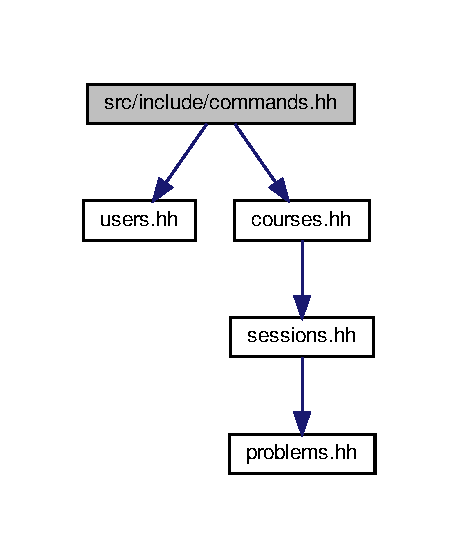
\includegraphics[width=220pt]{commands_8hh__incl}
\end{center}
\end{figure}
\subsection*{Classes}
\begin{DoxyCompactItemize}
\item 
class \hyperlink{classEvaluator}{Evaluator}
\begin{DoxyCompactList}\small\item\em Class that contains a deployable instance of the \hyperlink{classEvaluator}{Evaluator} Platform. \end{DoxyCompactList}\end{DoxyCompactItemize}


\subsection{Detailed Description}
\hyperlink{classEvaluator}{Evaluator} main program class. 

\begin{DoxyAuthor}{Author}
Ivan Cala Mesa 
\end{DoxyAuthor}
\begin{DoxyDate}{Date}
1st of April of 2021 
\end{DoxyDate}

\hypertarget{courses_8hh}{}\section{src/include/courses.hh File Reference}
\label{courses_8hh}\index{src/include/courses.\+hh@{src/include/courses.\+hh}}


\hyperlink{classCourse}{Course} class and its list interface.  


{\ttfamily \#include \char`\"{}sessions.\+hh\char`\"{}}\newline
Include dependency graph for courses.\+hh\+:
\nopagebreak
\begin{figure}[H]
\begin{center}
\leavevmode
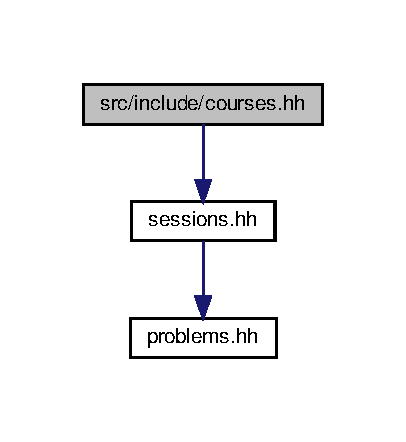
\includegraphics[width=195pt]{courses_8hh__incl}
\end{center}
\end{figure}
This graph shows which files directly or indirectly include this file\+:
\nopagebreak
\begin{figure}[H]
\begin{center}
\leavevmode
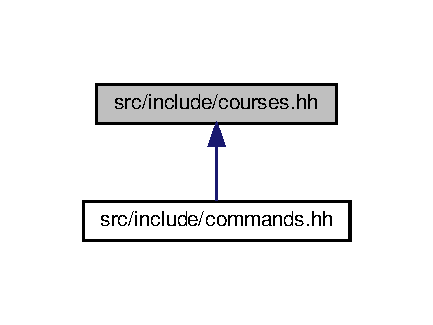
\includegraphics[width=208pt]{courses_8hh__dep__incl}
\end{center}
\end{figure}
\subsection*{Classes}
\begin{DoxyCompactItemize}
\item 
class \hyperlink{classCourse}{Course}
\begin{DoxyCompactList}\small\item\em Repository of \hyperlink{classSession}{Session} instances identified by an unique id. \end{DoxyCompactList}\item 
class \hyperlink{classCourses}{Courses}
\begin{DoxyCompactList}\small\item\em Interface of a repository of different courses, uniquely identified by their id. \end{DoxyCompactList}\end{DoxyCompactItemize}


\subsection{Detailed Description}
\hyperlink{classCourse}{Course} class and its list interface. 

\begin{DoxyAuthor}{Author}
Ivan Cala Mesa 
\end{DoxyAuthor}
\begin{DoxyDate}{Date}
1st of April of 2021 
\end{DoxyDate}

\hypertarget{problems_8hh}{}\section{src/include/problems.hh File Reference}
\label{problems_8hh}\index{src/include/problems.\+hh@{src/include/problems.\+hh}}


\hyperlink{classProblem}{Problem} class and a problem repository interface.  


This graph shows which files directly or indirectly include this file\+:
\nopagebreak
\begin{figure}[H]
\begin{center}
\leavevmode
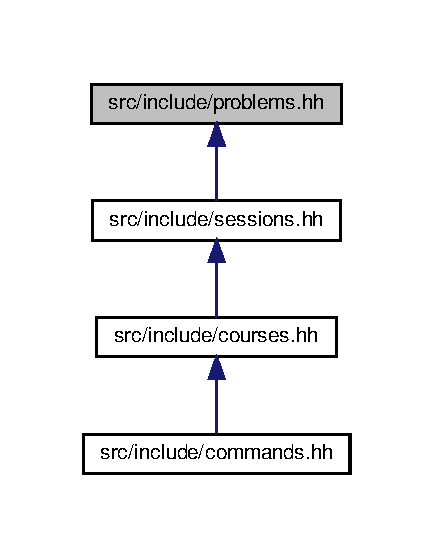
\includegraphics[width=208pt]{problems_8hh__dep__incl}
\end{center}
\end{figure}
\subsection*{Classes}
\begin{DoxyCompactItemize}
\item 
class \hyperlink{classProblem}{Problem}
\begin{DoxyCompactList}\small\item\em Class that behaves as an uniquely id-\/identified problem in the \hyperlink{classEvaluator}{Evaluator} platform. \end{DoxyCompactList}\item 
class \hyperlink{classProblem__repo}{Problem\+\_\+repo}
\begin{DoxyCompactList}\small\item\em General interface for a repository of \hyperlink{classProblem}{Problem} instances. \end{DoxyCompactList}\end{DoxyCompactItemize}


\subsection{Detailed Description}
\hyperlink{classProblem}{Problem} class and a problem repository interface. 

\begin{DoxyAuthor}{Author}
Ivan Cala Mesa 
\end{DoxyAuthor}
\begin{DoxyDate}{Date}
1st of April of 2021 
\end{DoxyDate}

\hypertarget{sessions_8hh}{}\section{src/include/sessions.hh File Reference}
\label{sessions_8hh}\index{src/include/sessions.\+hh@{src/include/sessions.\+hh}}


\hyperlink{classSession}{Session} class and the session list interface.  


{\ttfamily \#include \char`\"{}problems.\+hh\char`\"{}}\newline
Include dependency graph for sessions.\+hh\+:
\nopagebreak
\begin{figure}[H]
\begin{center}
\leavevmode
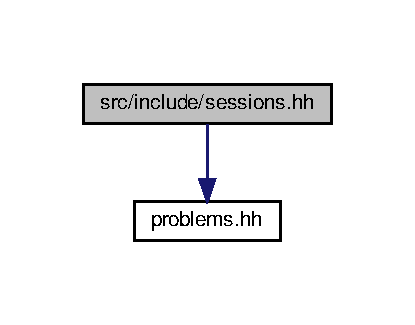
\includegraphics[width=199pt]{sessions_8hh__incl}
\end{center}
\end{figure}
This graph shows which files directly or indirectly include this file\+:
\nopagebreak
\begin{figure}[H]
\begin{center}
\leavevmode
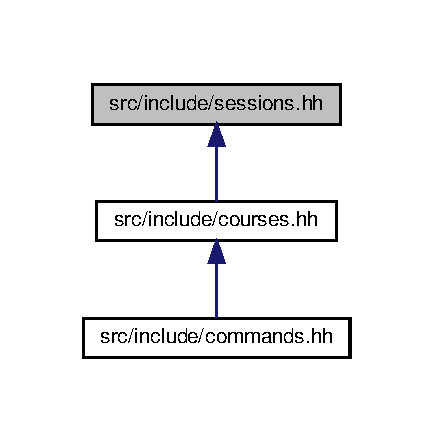
\includegraphics[width=208pt]{sessions_8hh__dep__incl}
\end{center}
\end{figure}
\subsection*{Classes}
\begin{DoxyCompactItemize}
\item 
class \hyperlink{classSession}{Session}
\begin{DoxyCompactList}\small\item\em Class that behaves as a problem set with completion requisites. \end{DoxyCompactList}\item 
class \hyperlink{classSessions}{Sessions}
\begin{DoxyCompactList}\small\item\em General interface to manage a \hyperlink{classSession}{Session} repository. \end{DoxyCompactList}\end{DoxyCompactItemize}


\subsection{Detailed Description}
\hyperlink{classSession}{Session} class and the session list interface. 

\begin{DoxyAuthor}{Author}
Ivan Cala Mesa 
\end{DoxyAuthor}
\begin{DoxyDate}{Date}
1st of April of 2021 
\end{DoxyDate}

\hypertarget{users_8hh}{}\section{src/include/users.hh File Reference}
\label{users_8hh}\index{src/include/users.\+hh@{src/include/users.\+hh}}


Specification of the whole User list/\+DB general-\/use interface.  


This graph shows which files directly or indirectly include this file\+:
\nopagebreak
\begin{figure}[H]
\begin{center}
\leavevmode
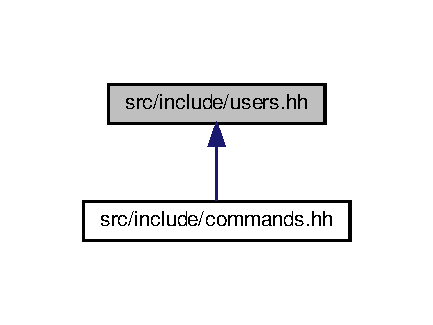
\includegraphics[width=208pt]{users_8hh__dep__incl}
\end{center}
\end{figure}
\subsection*{Classes}
\begin{DoxyCompactItemize}
\item 
class \hyperlink{classUsers}{Users}
\begin{DoxyCompactList}\small\item\em General interface to store and access the user list. \end{DoxyCompactList}\end{DoxyCompactItemize}


\subsection{Detailed Description}
Specification of the whole User list/\+DB general-\/use interface. 

Both User and \hyperlink{classUsers}{Users} are \textquotesingle{}independent\textquotesingle{} classes in that they do not require any other class to make sense as a whole. In this case, especially the User class is an self-\/contained class (even its id is inside it). \begin{DoxyAuthor}{Author}
Ivan Cala Mesa 
\end{DoxyAuthor}
\begin{DoxyDate}{Date}
1st of april of 2021 
\end{DoxyDate}

%--- End generated contents ---

% Index
\backmatter
\newpage
\phantomsection
\clearemptydoublepage
\addcontentsline{toc}{chapter}{Index}
\printindex

\end{document}
